\begin{example} \label{eg:6.3.4} % EXAMPLE
Find the surface area of the solid formed by revolving $y=\sin x$ on $[0,\pi]$ around the $x$-axis, as shown in Figure \ref{F:6.3.Ex4}.

\solution
The setup is relatively straightforward; we have the surface area $SA$ is:
\begin{align*}
SA  &=	2\pi\int_0^\pi \sin x\sqrt{1+\cos^2x}\ dx \\
	&= 2\pi \int_{-1}^1 \sqrt{1+u^2} \ du \\
		&=	2\pi \int_{-\pi/4}^{\pi/4} \sec^3\theta \ d\theta \\
		&= 2\pi\sqrt{2}.		
\end{align*}
The integration above is nontrivial, utilizing Substitution, Trigonometric Substitution, and Integration by Parts.
\end{example}

\begin{marginfigure}[-8cm] %MARGIN FIGURE
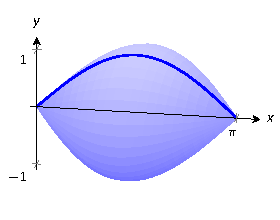
\includegraphics{figures/figsa1}
\caption{Revolving $y=\sin x$ on $[0,\pi]$ about the $x$-axis.} \label{F:6.3.Ex4}
\end{marginfigure}



